\chapter{Random Number Generation} \label{sec:fingerprints}

\section{Theory and Implementation}

This section describes techniques to generate unique fingerprints from Flash memory devices.

\subsection{Sources of Uniqueness}

Flash memory is subject to random process variation like any other semiconductor device. Because Flash is fabricated for maximum density, small variations can be significant. Process variation can cause each bit of a Flash memory to differ from its neighbors. While variation may affect many aspects of Flash cells, our fingerprinting technique exploits threshold voltage variations. Variations in doping, floating gate oxide thickness, and control-gate coupling ratio can cause the threshold voltage of each transistor to vary. Because of this threshold voltage variation, different Flash cells will need different times to be programmed.

\subsection{Extracting Fingerprints}

In this paper, we introduce a fingerprinting scheme based on partial programming. We repeatedly partially program a page on a Flash chip. After each partial program, some bits will have been programmed enough to flip their states from 1 to 0. For each bit in the page, we record the order in which the bit flipped. Pseudo-code is provided in Algorithm V. In our experiments, T is chosen to be 29.3us. A short partial program time provide a better resolution to distinguish different bits with the cost of increased fingerprinting time. We do not enforce all bits to be programmed, in order to account for the possibility of faulty bits.

\begin{figure} 
\begin{center} 

%\begin{scriptsize}
\begin{center}

\begin{tabular}{|c|}
\hline
\begin{minipage}[t]{3.2in}



\begin{tabbing}
{\bf Algorithm V  Extract the order in which bits in a page }
\\ {\bf reach the programmed state. }
\\
\\ Choose a partial programming time T (below the 
\\ rated program time). 
\\
\\ Nbits = number of bits in one page
\\ Order = 1; 
\\ Initialize BitRank[Nbits] to 0.
\\
\\ {\bf do} \= \{
\\ \>    Partially program a page for T;
\\ \>    {\bf For} \= all programmed bits {\bf do}
\\ \>\>        BitRank[programmed bit] = Order;
\\ \>    {\bf End for}
\\ \>    Order = Order + 1;
\\ \} repeat until most (99\%) bits in the page are programmed 


\end{tabbing}
\end{minipage}
\\ \hline
\end{tabular}
\end{center}
%\end{scriptsize}
 
\caption{Extract the order in which bits in a page reach the programmed state.}
\label{fig:extract_order} 
\vspace{-0.25in}
\end{center} 
\end{figure}

\subsection{Comparing Fingerprints}

The fingerprints extracted from the same page on the same chip over time are noisy but highly correlated. To compare fingerprints extracted from the same page/chip and different pages/chips, we use the Pearson correlation coefficient \cite{trust2011}, which is defined as

\begin{equation}
P(x,y)=\frac{E[(X-\mu_X)(Y-\mu_Y)]}{\sigma_X\sigma_Y}
\end{equation}

where X is the vector of program orders extracted from one experiment and Y is another vector of program orders extracted from another experiment. $\mu_X$ and $\sigma_X$ are the mean and standard deviation of the X vector. $\mu_Y$ and $\sigma_Y$ are the mean and standard deviation of the Y vector. 

In this way, the vector of program orders is treated as a vector of realizations of a random variable. For vectors extracted from the same page, $Y=aX+b+noise$ where a and b are constants and the noise is small. So, X and Y are highly correlated and the correlation coefficient should be close to 1. For vectors extracted from different pages, X and Y should be nearly independent of each other, so the correlation coefficient should be close to zero. From another perspective, if both X[i] and Y[i] are smaller or bigger than their means, $(X[i]-\mu_X)(Y[i]-\mu_Y)$ would be a positive number. If not, it would be a negative number. If X and Y are independent, it is equally likely to be positive and negative so the correlation coefficient would approach 0.

\begin{figure}
  \centering
  \subfigure[][]{
    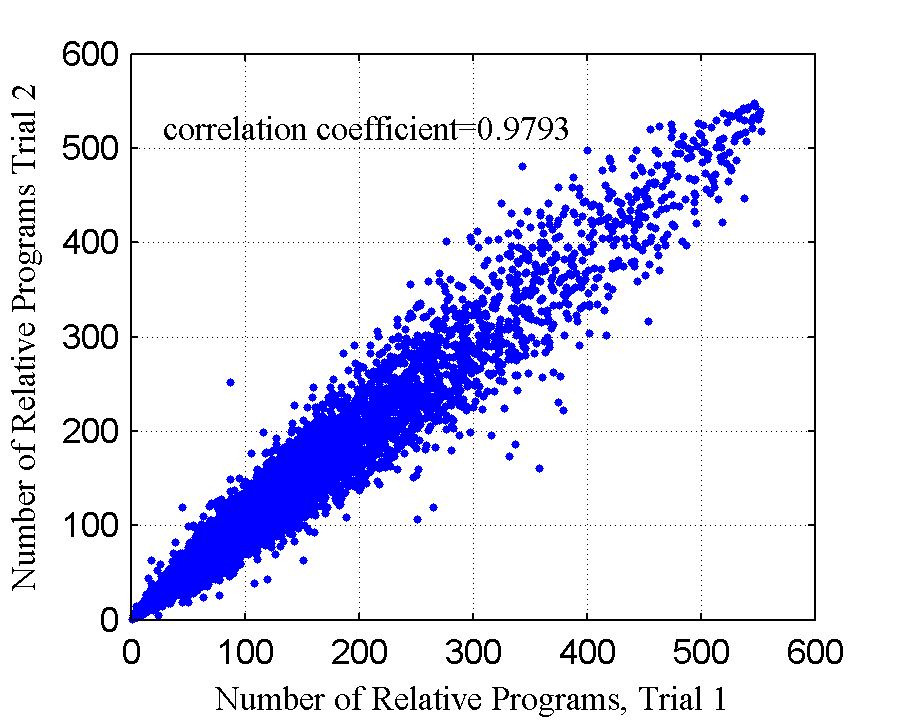
\includegraphics[width=\mywidth]{figs/fprints_same_page.png}
    \label{fig:fprints_same_page}
  }
  
  \subfigure[][]{
    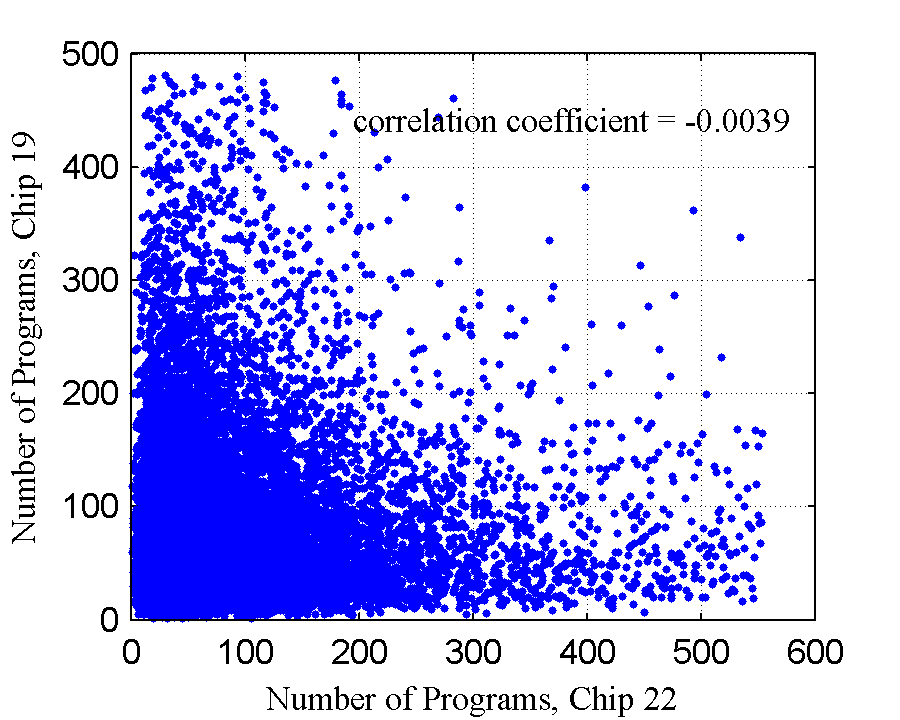
\includegraphics[width=\mywidth]{figs/fprints_diff_page.png}
    \label{fig:fprints_diff_page}
  }
  \caption{Scatter plot for fingerprints extracted on (a) the same page and (b) different chips.}
  \label{fig:fprints_scatter}
\end{figure}

The scatter plot of X and Y from the same page/chip and from different chips are shown in Figure~\ref{fig:fprints_scatter}. The figure clearly demonstrates a high correlation between fingerprints from the same chip over time and a low correlation between fingerprints from different chips. Therefore, this correlation metric can be used to compare fingerprints to determine whether they are from the same page/chip or from different pages/chips.

\subsection{Fingerprints in Binary Numbers}

The above fingerprints are in the form of the order in which each bit was programmed. If an application requires a binary number such as in generating cryptographic keys, we need to convert the recorded ordering into a binary number.

There are a couple of ways to generate unique and unpredictable binary numbers from the Flash fingerprints. First, we can use a threshold to convert a fingerprint based on the programming order into a binary number as shown in Algorithm VI. In the algorithm, we produce 1 if the program order is high, or 0 otherwise. This approach produces a 1 bit fingerprint for each Flash bit. Alternatively, we can obtain a similar binary fingerprint directly from Flash memory by partially programming (or erasing) a page and reading bits (1/0) from the Flash.

\begin{figure} 
\begin{center} 

%\begin{scriptsize}
\begin{center}

\begin{tabular}{|c|}
\hline
\begin{minipage}[t]{3.2in}



\begin{tabbing}
{\bf Algorithm VI  Generate a binary signature from the partial  }
\\ {\bf programming order information. }
\\
\\ Pick threshold $t = Max(BitRank) / 2$
\\ {\bf For} \= each bit
\\ \>    {\bf If} \= $BitRank[bit] > t$
\\ \>\>       Output 1
\\ \>    {\bf Else} Output 0
\\ {\bf End for}


\end{tabbing}
\end{minipage}
\\ \hline
\end{tabular}
\end{center}
%\end{scriptsize}
 
\caption{Generate a binary signature from the partial programming order information.}
\label{fig:gen_signature} 
\vspace{-0.25in}
\end{center} 
\end{figure}

\section{Evaluation}
 
The experiment setup and tested devices are the same as in the previous chapter. 

For fingerprinting, we are interested in uniqueness and robustness of fingerprints. The fingerprint should be unique, which means that fingerprints from different chips or different locations of the same chip must be significantly different – the correlation coefficient should be low. The fingerprint should also be robust, in a sense that fingerprints from a given location of a chip must stay stable over time and even under different environmental conditions – the correlation coefficient should be high.

In the experiments detailed below, we used 24 chips (Micron 34nm SLC), and 24 pages (6 pages in 4 blocks) from each chip. 10 measurements were made from each page. Each page has 16,384 bits.

\subsection{Uniqueness}

To test uniqueness, we compared the fingerprint of a page to the fingerprints of the same page on different chips, and recorded their correlation coefficients. A total of 66,240 pairs were compared – (24 chips choose 2) * 24 pages * 10 measurements. The results are shown in Figure~\ref{fig:fprints_histo_diff_chip}. The correlation coefficients are very low, with an average of 0.0076. A Gaussian distribution fits the data well, as shown in red.

\begin{figure}
\begin{center} 
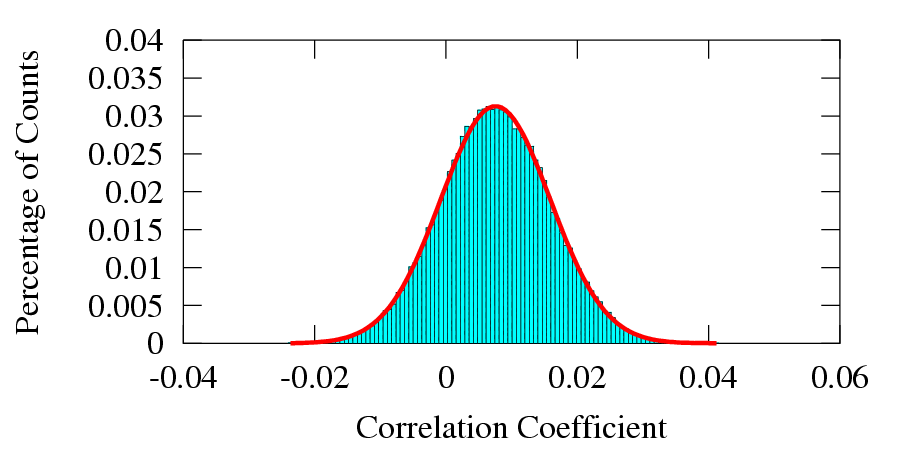
\includegraphics[width=\mywidth]{figs/fprints_histo_diff_chip.png} 
\caption{Histogram of correlation coefficients for pages compared to the same page on a different chip (total 66,240 comparisons).}
\label{fig:fprints_histo_diff_chip} 
\vspace{-0.1in}
\end{center} 
\end{figure} 

The correlation coefficients are also very low when a page is compared not only to the same page on different chips, but also to different pages on the same and different chips, shown in Figure~\ref{fig:fprints_histo_diff_page}. There are 1,656,000 pairs in comparison – ((24 pages * 24 chips) choose 2) * 10 measurements. This indicates that fingerprints from different parts (pages) of a chip can be considered as two different fingerprints and do not have much correlation. Therefore, the fingerprinting scheme allows the generation of many independent fingerprints from a single chip. The average correlation coefficient in this case is 0.0072.


\begin{figure}
\begin{center} 
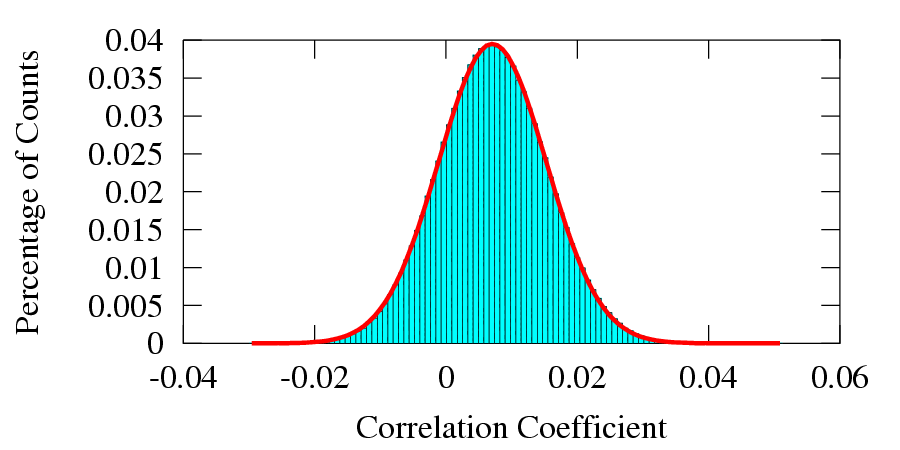
\includegraphics[width=\mywidth]{figs/fprints_histo_diff_page.png} 
\caption{Histogram of correlation coefficients for every page compared to every other page at room temp (total 1,656,000 comparisons).}
\label{fig:fprints_histo_diff_page} 
\vspace{-0.1in}
\end{center} 
\end{figure} 

\subsection{Robustness}

To test robustness, we compared each page’s measurement to the 9 other measurements of the same page’s fingerprint (an intra-chip measurement). The histogram of results for all pages is shown in Figure~\ref{fig:fprints_histo_same_page}. The correlation coefficient for fingerprints from the same page is very high, with an average of 0.9673. The minimum observed coefficient is 0.9022. The results show that fingerprints from the same page are robust over multiple measurements, and can be easily distinguished from fingerprints of a different chip or page. 

To be used in an authentication scheme, one could set a threshold correlation coefficient t. If, when comparing two fingerprints, their correlation coefficient is above t, then the two fingerprints are considered to have come from the same page/chip. If their correlation coefficient is below t, then the fingerprints are assumed to be from different pages/chips. 

\begin{figure}
\begin{center} 
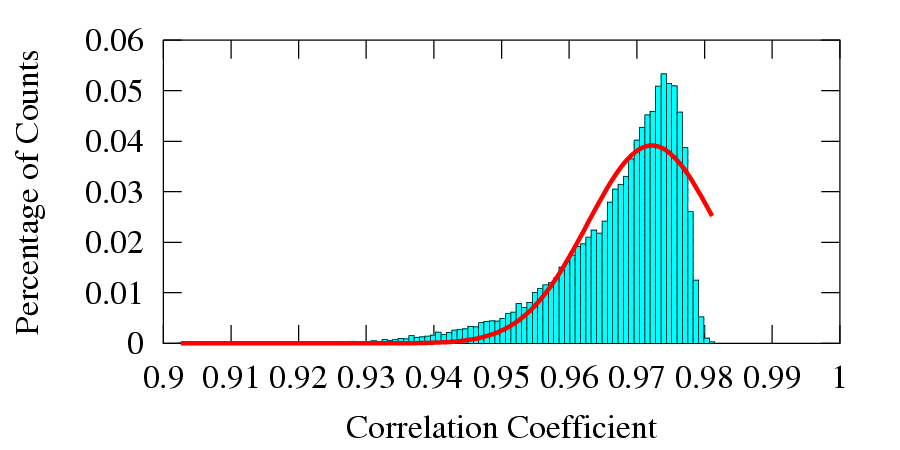
\includegraphics[width=\mywidth]{figs/fprints_histo_same_page.png} 
\caption{Histogram of correlation coefficients for all intra-chip comparisons (total 25,920 comparisons).}
\label{fig:fprints_histo_same_page} 
\vspace{-0.1in}
\end{center} 
\end{figure} 

In such a scheme, there is a potential concern for false positives and false negatives. A false negative is defined as comparing fingerprints that are actually from two different pages/chips, but deciding that the fingerprints are from the same page/chip. A false positive occurs when comparing fingerprints from the same page/chip, yet deciding that the fingerprints came from two different pages/chips. The threshold t can be selected to balance false negatives and positives. A high value of t would minimize false negatives, but increase the chance of false positives, and vice versa.

To estimate the chance of false positives and false negatives, we fit normal probability mass distribution functions to the correlation coefficient distribution. A false positive would arise from a comparison of two fingerprints from the same page being below t. The normal distribution fitted to the intra-chip comparison data in Figure~\ref{fig:fprints_histo_same_page} has an average $\mu = 0.9722$ and a std. deviation of 0.0095. For a threshold of $t = 0.5$, the normal distribution function estimates the cumulative probability of a pair of fingerprints having a correlation coefficient below 0.5 as $2.62*10^{539}$. At t = 0.7, the probability is estimated as $7.43*10^{-181}$.

The normal distribution function fitted to the inter-chip comparison data in Figure~\ref{fig:fprints_histo_diff_page} has a $\mu = 0.0076$ and a std. deviation of 0.0083. The estimated chance of a pair of fingerprints from different chips exceeding $t = 0.5$ is $4.52*10^{-815}$. At $t = 0.3$, the probability is estimated as $6.14*10^{-301}$.

The tight inter-chip and intra-chip correlations along with low probability estimates for false positives or negatives suggest that the size of fingerprints can possibly be reduced. Instead of using all 16,384 bits in a page, we can generate a fingerprint for a 1024-bit, 512-bit, or even only a 256-bit block. Experiments show that the averages of the observed correlation coefficients remain similar to those when using every bit in a page while the standard deviation increases by a factor of 2-3. However, the worst-case false negative estimates remain low. When using 256 bit fingerprints with the threshold $t = 0.3$, the estimate is $7.91*10^{-7}$. Under the same conditions, using 1024 bit fingerprints gives an estimated $3.20*10^{-22}$ chance of a false negative.

\subsection{Temperature Variations and Aging}

To see how robust the fingerprints are across different temperatures. We extracted fingerprints from chips at two other ambient temperatures, 60 °C and -5 °C. We tested a subset of the chips tested at room temperature – 6 pages (3 pages in 2 blocks) in 6 chips. 

Of interest is how fingerprints from the same page/chip, but taken at different temperatures, compare. Figure~\ref{fig:fprints_temp} shows the results of the intra-chip comparison between each temperature pair. Correlations remain high for fingerprints from the same page/chip, indicating that fingerprints taken at different temperatures can still be identified as the same. The average correlation coefficient is lower than when compared without a temperature difference, but is still sufficiently high to have very low false positive rates.

\begin{figure}
\begin{center} 
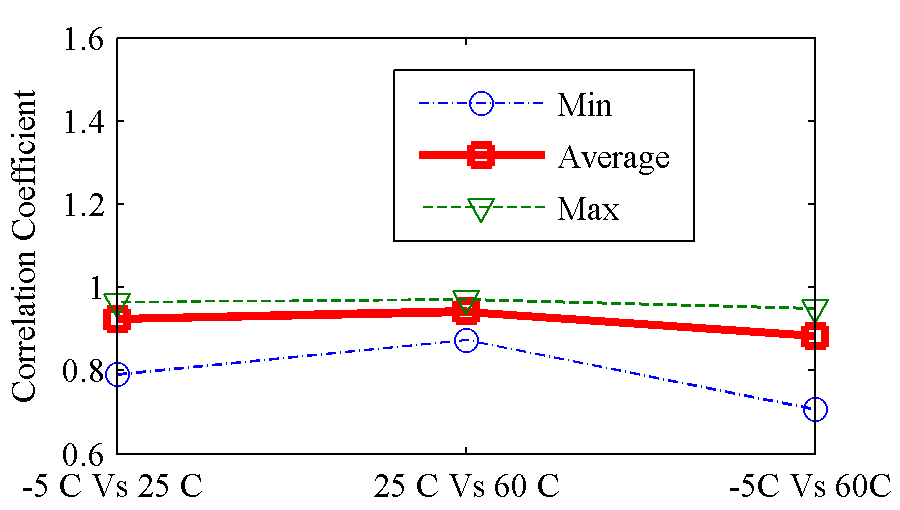
\includegraphics[width=\mywidth]{figs/fprints_temp.png} 
\caption{Average, minimum, and maximum correlation coefficients for intra-chip comparisons between different ambient temperatures.}
\label{fig:fprints_temp} 
\vspace{-0.1in}
\end{center} 
\end{figure} 

Comparing fingerprints from the same page at the same temperature at -5 °C or 60 °C still yields high correlation coefficients, as expected. Comparisons of fingerprints from different pages/chips at different temperatures give very low correlation coefficients.

\begin{figure}
\begin{center} 
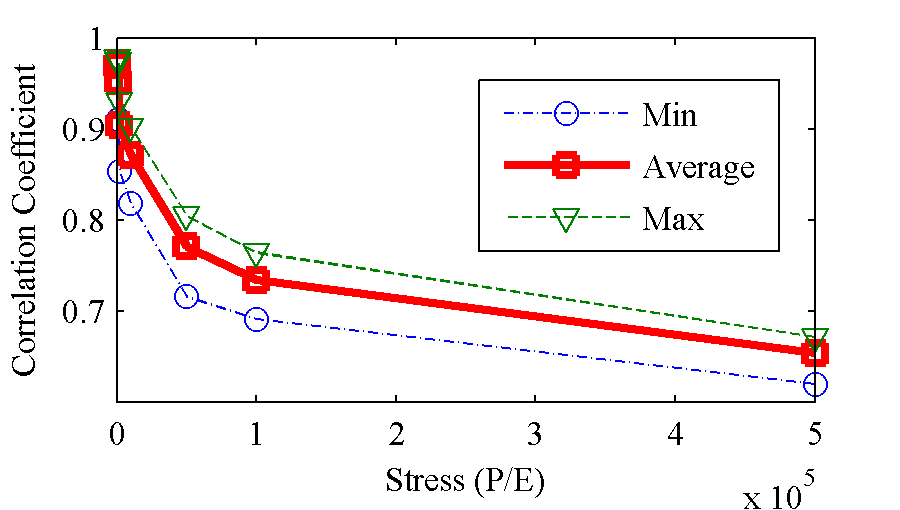
\includegraphics[width=\mywidth]{figs/fprints_aging.png} 
\caption{Average, minimum, and maximum correlation coefficients for comparisons between fresh and stressed Flash.}
\label{fig:fprints_aging} 
\vspace{-0.1in}
\end{center} 
\end{figure} 

Flash chips have a limited lifetime, wearing out over many program/erase (P/E) cycles. For a page’s fingerprint to be useful over time, fingerprints taken later in life should still give high correlation with younger fingerprints. Figure~\ref{fig:fprints_aging} shows the results of comparing fingerprints for the same page/chip taken when a Flash chip is new to fingerprints taken after a different number of P/E cycles. While the average correlation coefficient goes down noticeably, we note that it appears to bend towards an asymptote as the chip wears out. Even after 500,000 P/E cycles, which is beyond the typical lifetime of Flash chips, the average coefficient is still high enough to distinguish fingerprints of the same page/chip from fingerprints acquired from a different page/chip.

However, we found that an extreme wear-out such as 500,000 P/E cycles can raise a non-negligible false positive concern $(10^{-4})$ for short 256 or 512-bit fingerprints. This result indicates that we need longer fingerprints if they need to be used over a long period of time without a re-calibration.

\subsection{Security}

An attacker could attempt to store the fingerprints of a Flash device and replay the fingerprint to convince a verifier that he has the Flash chip in question. If the attacker cannot predict which page(s) or parts of a page (for shorter signatures) will be fingerprinted, he would need to store the fingerprints for every page to ensure success. The Flash chips in our experiments required about 800 partial program cycles per fingerprint. As the fingerprint comprises the order in which the bit was programmed, each bit’s ordering could be stored as a 10-bit number. To store an entire chip’s fingerprints would require 10x the chip storage. 

Acquiring a single fingerprint is relatively fast. Our setup could record an entire page’s fingerprint in about 10 seconds. However, there are 131,072 pages on our (relatively small) test chip; characterizing one chip would take about 2 weeks. The characterization time depends on the speed of the Flash interface, and we plan to further investigate the limit on how fast fingerprints can be characterized. 

\subsection{Applicability to Multiple Flash Chips}

Most of the above experimental results are obtained from the Micron SLC Flash memory. In order to answer the question of whether the proposed techniques are applicable to Flash memory in general, we have repeated both RNG and fingerprinting tests on four types of Flash memory chips in Table~\ref{tab:testedchips}, including an MLC chip.

The experiments showed that RNG and fingerprinting both work on all four types of Flash chips, with comparable performance. Detailed results are not included as they do not add new information. 

While we found that the proposed algorithm works without any change in most cases, there was one exception where the fingerprinting algorithm needed to be slightly modified in order to compensate for systematic variations for certain manufacturers. For example, for the Hynix and Numonyx chips, we found that bits from the even bytes of a page tend to be programmed quicker than bits from the odd bytes. Similarly, for the MLC chip, bits in a page divide into two groups: a quickly programmed group and a slowly programmed group. To accommodate such systematic behaviors, the fingerprinting algorithm was changed to only compare programming ordering of bits within the same group. 

\section{Application Scenarios}

One application of the Flash device fingerprints is to identify and/or authenticate hardware devices themselves similar to the way that we use biometrics to identify humans.

As an example, let us consider distinguishing genuine Flash memory chips from counterfeits through an untrusted supply chain. Recent articles report multiple incidents of counterfeit Flash devices in practice, such as chips from low-end manufacturers, defective chips, and ones harvested from thrown-away electronics, etc. \cite{trust2011, eetimesfakeparts, sosfakeflash}. The counterfeit chips cause a serious concern for consumers in terms of reliability as well as security; counterfeits may contain malicious functions. Counterfeits also damage the brand name for a manufacturer.

The Flash fingerprints can enable authentication of genuine chips without any additional hardware modifications to today’s Flash chips. In a simple protocol, a Flash manufacturer can put an identifier (ID) to a genuine chip (write to a location in Flash memory), generate a fingerprint from the chip, and store the fingerprint in a database along with the ID. To check the authenticity of a Flash chip from a supply chain, a customer can regenerate a fingerprint and query the manufacturer’s database to see if it matches the saved fingerprint. 

In order to pass the check, a counterfeit chip needs to produce the same fingerprint as a genuine one. Interestingly, unlike simple identifiers and keys stored in memory, device fingerprints based on random manufacturing variations cannot be controlled even when a desired fingerprint is known. For example, even legitimate Flash manufacturers cannot precisely control individual transistor threshold voltages, which we use to generate fingerprints. To produce specific fingerprints, one will need to create a custom chip that stores the fingerprints and emulates Flash responses.

The authentication scheme can be strengthened against emulation attacks by exploiting a large number of bits in Flash memory.  Figure~\ref{fig:auth_app} illustrates a modified protocol that utilizes a large number of fingerprints that can be generated from each Flash chip. Here, we consider a Flash chip as a function where a different set of bits that are used to generate a fingerprint is a challenge, and the resulting fingerprint is a response. A device manufacturer, when in possession of a genuine IC, applies randomly chosen challenges to obtain responses. Then, these challenge-response pairs (CRP) are stored in a database for future authentication operations. To check the authenticity of an IC later, a CRP that has been previously recorded but has never been used for a check is selected from the database, and a re-generated response from a device can be checked.

\begin{figure}
\begin{center} 
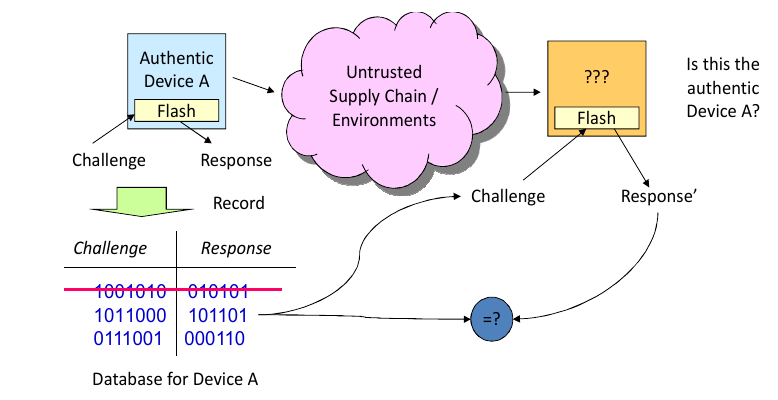
\includegraphics[width=\mywidth]{figs/authentication_app.png} 
\caption{Device authentication through a challenge-response protocol.}
\label{fig:auth_app} 
\vspace{-0.1in}
\end{center} 
\end{figure} 

Unless an adversary can predict which CRPs will be used for authentication, the adversary needs to measure all (or at least a large fraction) of possible fingerprints from an authentic Flash chip and store them in an emulator. In our prototype board, a generation of all fingerprints from a single page (16K bits) takes about 10 seconds and requires 10 bits of storage for each Flash bit. For a 16Gbit (2 GB) Flash chip, which is a moderate size by today’s standards, this implies that fully characterizing the chip will take hundreds of days and 20 GB storage. In the context of counterfeiting, such costs are likely to be high enough to make producing counterfeits economically unattractive. 

The security of the authentication scheme based on Flash fingerprints can be further improved if an additional control can be added to the Flash interface. For example, imagine using a USB Flash memory as a two-factor authentication token by updating its firmware to have a challenge-response interface for Flash fingerprints. Given that authentication operations only need to be infrequent, the USB stick can be configured to only allow a query every few seconds. If a fingerprint is based on 1024 Flash bits, fully characterizing an 8 GB USB stick can take tens of years.

In addition to device identification and authentication, the Flash fingerprints can be used as a way to produce many independent secret keys without additional storage. In effect, the proposed Flash fingerprints provide unpredictable and persistent numbers for each device. Previous studies such as fuzzy extractors \cite{dodis2004fuzzy} and Physical Unclonable Functions (PUFs) \cite{suhpuf2007} have shown how symmetric keys (uniformly distributed random numbers) can be obtained from biometric data or IC signatures from manufacturing variations by applying hashing and error correction. The same approach can be applied to Flash fingerprints in order to generate reliable cryptographic keys. A typical Flash with a few GB can potentially produce tens of millions of 128-bit symmetric keys.

\section{Related Work}

Instead of conventional authentication based on a secret key and cryptographic computation, researchers have recently proposed to use the inherent variation in physical characteristics of a hardware device for identification and authentication. Process variation in semiconductor foundries is a common source of hardware uniqueness which is out of the control of the designer \cite{boning1996statistical, bowman2002impact, nassif2000modeling}. A unique fingerprint can be extracted and used to identify the chip, but cannot be used for security applications because it can be simply stored and replayed. We also take advantage of process variation for our fingerprinting scheme. 
For security applications, Physical Unclonable Functions (PUFs) have been proposed. A PUF can generate many fingerprints per device by using complex physical systems whose analog characteristics cannot be perfectly replicated. Pappu initially proposed PUFs \cite{ravikanth2001physical} using light scattering patterns of optically transparent tokens. In silicon, researchers have constructed circuits which, due to random process variation, emit unique outputs per device. Some silicon PUFs use ring oscillators \cite{gassend2002silicon} or race conditions between two identical delay paths \cite{lee2004technique}. These PUFs are usually implemented as custom circuits on the chip. Recently, PUFs have been implemented without additional circuitry by exploiting metastable elements such as SRAM cells, which have unique value on start-up for each IC instance \cite{koeberl2011practical, holcomb2007initial}, or in Flash memories \cite{trust2011}. 
Our authentication scheme requires no new circuitry and can be done with commercially available and ubiquitous Flash chips. Unlike metastable elements, authentication does not require a power cycle. The scheme can generate many fingerprints by using more pages in the Flash chip. Acquiring a fingerprint is also faster and more widely applicable than previous Flash authentication methods.